\section{Lösung von Nullstellenproblemen}

\subsection{Problemstellung NSP}

Eine Gleichung der Form $F(x)=x$ heisst Fixpunktgleichung.

\begin{itemize}
  \item Ihre Lösungen $\bar{x}$, für die $F(\bar{x})=\bar{x}$ erfüllt ist, heissen Fixpunkte.
\end{itemize}

\subsection{Fixpunktiteration}

Gegeben sei $F:[a, b] \rightarrow \mathbb{R}$, mit $x_{0} \in[a, b]$. Die rekursive Folge

$$
x_{x+1} \equiv F\left(x_{n}\right), \quad n=0,1,2, \ldots
$$

Heisst Fixpunktiteration von $F$ zum Startwert $x_{0}$.\\
Sei $F:[a, b] \rightarrow \mathbb{R}$ mit stetiger Ableitung $F^{\prime}$ und $\bar{x} \in[a, b]$ ein Fixpunkt von $F$. Dann gilt für die Fixpunktiteration $x_{n+1}=F\left(x_{n}\right)$

\begin{itemize}
  \item $\quad\left|F^{\prime}(\bar{x})\right|<1 \quad x_{n}$ konvergiert gegen $\bar{x}$, falls $x_{0}$ nahe genug bei $\bar{x}$ liegt anziehend
  \item $\left|F^{\prime}(\bar{x})\right|>1 \quad x_{n}$ konvergiert für keinen Startwert $x_{0} \neq \bar{x}$ abstossend
\end{itemize}

\section*{Banachscher Fixpunktsatz}
Sei $F:[a, b] \rightarrow[a, b]$ und es existiere eine Konstante $\alpha$, wobei gilt

\begin{itemize}
  \item $\alpha(0<\alpha<1)$ : Lipschitz-Konstante
  \item $\forall_{x, y}(x, y \in[a, b])$
\end{itemize}

$$
|F(x)-F(y)| \leq \alpha|x-y|, \quad \frac{|F(x)-F(y)|}{|x-y|} \leq \alpha
$$

Dann gilt

\begin{itemize}
  \item $\quad F$ hat genau einen Fixpunkt $\bar{x}$ in $[a, b]$
  \item Die Fixpunktiteration $x_{n+1}=F\left(x_{n}\right)$ konvergiert gegen $\bar{x}$ für alle Startwerte $x_{0} \in[a, b]$
  \item Es gelten die Fehlerabschätzungen
  \item $\left|x_{n}-\bar{x}\right| \leq \frac{\alpha^{n}}{1-\alpha} \cdot\left|x_{1}-x_{0}\right| \quad$ a-priori Abschätzung
  \item $\left|x_{n}-\bar{x}\right| \leq \frac{\alpha}{1-\alpha} \cdot\left|x_{n}-x_{n-1}\right| \quad$ a-posteriori Abschätzung
\end{itemize}

Berechne die Nullstellen von $p(x)=x^{3}-x+0.3$\\
Fixpunktiteration

$$
x_{n+1}=F\left(x_{n}\right)=x_{n}^{3}+0.3
$$

$F\left(x_{n}\right)$ steigt stetig an\\
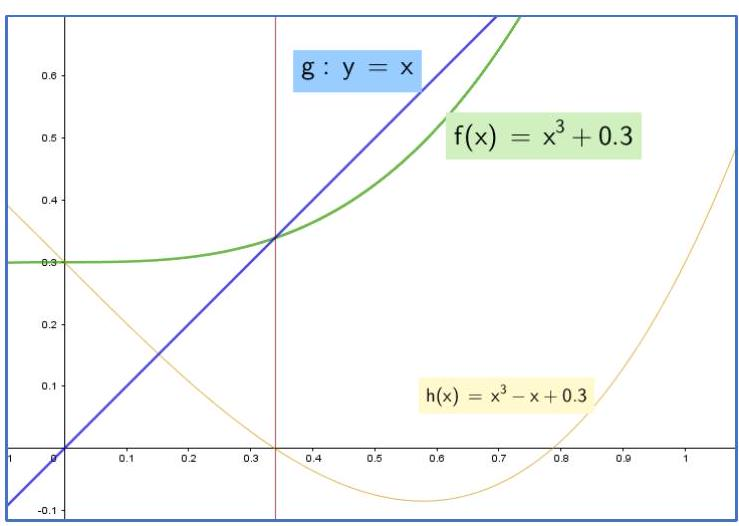
\includegraphics[width=\linewidth]{images/2024_12_29_68ccba06d0091c162fa4g-02}\\
$F: I \rightarrow I$ gilt wenn...

$$
F(a)>a, \quad F(b)<b
$$

Alpha bestimmen / überprüfen

$$
\alpha=\max _{x \in I}\left|F^{\prime}(x)\right| \leq 1
$$

Anzahl Iterationen $n$ berechnen

$$
n \geq \frac{\ln \left(\frac{t o l \cdot(1-\alpha)}{\left|x_{1}-x_{0}\right|}\right)}{\ln \alpha}
$$

\subsection{Newton-Verfahren}

Sukzessive Approximation der Funktionskurve $y=f(x)$ durch Tangenten, deren Schnittpunkt mit der x-Achse problemlos berechnet werden kann

Lösung $\xi$ der Gleichung $f(x)=0$ finden.\\
$>$ Startwert $x_{0}$ geeignet wählen (nahe bei $\xi$ )\\
$>$ Iterationsvorschrift:

$$
x_{n+1}=x_{n}-\frac{f\left(x_{n}\right)}{f^{\prime}\left(x_{n}\right)}
$$

Die Folge $\left(x_{n}\right)_{n \in \mathbb{N}}$ konvergiert gegen die Lösung $\xi$ der Gleichung $f(x)=0$.\\
$\left(x_{0}, x_{1}, x_{2}, \ldots\right)$ ist sicher gegeben, wenn im Intervall $[a, b]$, in dem alle Näherungswerte (und die Nullstellen selbst) liegen sollen, die Bedingung

$$
\left|\frac{f(x) \cdot f^{\prime \prime}(x)}{\left[f^{\prime}(x)\right]^{2}}\right|<1
$$

Erfüllt ist (hinreichende Konvergenzbedingung).

\section*{Vereinfachtes Newton-Verfahren}
Statt in jedem Schritt $f^{\prime}\left(x_{n}\right)$ auszurechnen, kann man immer wieder $f^{\prime}\left(x_{0}\right)$ verwenden.

$$
x_{n+1}=x_{n}-\frac{f\left(x_{n}\right)}{f^{\prime}\left(x_{0}\right)}
$$

\section*{Sekantenverfahren}
Der Schnittpunkt von Sekanten durch jeweils zwei Punkte $\left(x_{0}, f\left(x_{0}\right)\right)$ und $\left(x_{1}, f\left(x_{1}\right)\right)$ mit der $x$-Achse, wird berechnet.

$$
x_{n+1}=x_{n}-\frac{x_{n}-x_{n-1}}{f\left(x_{n}\right)-f\left(x_{n-1}\right)} \cdot f\left(x_{n}\right)
$$

\subsection{Konvergenzgeschwindigkeit}

Sei $\left(x_{n}\right)$ eine gegen $\bar{x}$ konvergierende Folge. Dann hat das Verfahren die Konvergenzordnung $q \geq 1$ wenn es eine Konstante $c>0$ gibt mit

$$
\left|x_{n+1}-\bar{x}\right| \leq c \cdot\left|x_{n}-\bar{x}\right|^{q}
$$

Für alle $n$.

\begin{itemize}
  \item $q=1 \quad$ lineare Konvergenz $\quad$ verlangt man noch $c<1$.
  \item $q=2$ quadratische Konvergenz
\end{itemize}

\subsection{Fehlerabschätzung}

Nullstellensatz von Bolzano\\
Sei $f:[a, b] \rightarrow \mathbb{R}$ stetig mit $f(a) \leq 0 \leq f(b)$ oder $f(a) \geq 0 \geq f(b)$. Dann muss $f$ in $[a, b]$ eine Nullstelle besitzen.

Sei $x_{n}$ also ein iterativ bestimmter Näherungswert einer exakten Nullstelle $\xi$ der stetigen Funktion $F: \mathbb{R} \rightarrow \mathbb{R}$ und es gelte für ein vorgegebene Fehlerschranke / Fehlertolerant $\epsilon>0$

$$
f\left(x_{n}-\epsilon\right) \cdot f\left(x_{n}+\epsilon\right)<0
$$

Dann muss gemäss dem Nullstellensatz im offenen Intervall $\left(x_{n}-\epsilon, x_{n}+\epsilon\right)$ eine Nullstelle $\xi$ liegen und es gilt die Fehlerabschätzung

$$
\left|x_{n}-\xi\right|<\epsilon
$$